\section{Algorithm}\label{sec:algorithm}

To clarify how we intend our approach to actually work we clarify concepts such as Road types, how protection schemes will be chosen, and how exactly we intend to apply the spatial and temporal anonymity of \tanonns. 

We will additionally present a set of algorithms to show how we intend our approach to handle the anonymization process.



\subsection{Applicability of Protection Schemes}

When users choose a classification for a \poi the system will attempt to automatically make some choices with regards to what the best way to anonymize that \poins. These choices are presented in table~\ref{tab:poitype} where it is shown which protection scheme(s) (Sec.~\ref{subsec:schemes}) is applicable for each classification. The trajectories will be sorted based on the classification of the \poi specifying sensitivity of its edges (possibly one trajectory will be have sub-trajectories sorted into multiple groups).

The first classification: "Public Service Point" is straight forward, the \ac{AS} scheme will always be chosen as the classification covers hospitals, clinics and the like, and thus always will be sensitive. 

The second classification is "House" which covers homes or institutions (e.g. a kindergarden). These will either only be sensitive on a one time basis i.e. use the \ac{RS} scheme, or only be sensitive at specific times when arriving or departing, leading to the \ac{ASTI} scheme.

\begin{table}[Htb]
\center
\begin{tabular}{|l|l|l|}
\hline
\bf Classification	& \bf Scheme \\\hline		
Public Service Point	& \ac{AS} \\\hline
House			& \ac{ASTI}, \ac{RS} \\\hline
Route w. endpoints	& \ac{AS}, \ac{ASTI}, \ac{RS}  \\\hline
Route w/o endpoints	& \ac{AS}, \ac{ASTI}, \ac{RS}  \\\hline

\end{tabular}
\caption{Applicability of protection schemes and types for different \poisns} 
\label{tab:poitype}
\end{table}



\subsection{Road Types} \label{subsec:roadtypes}

\rt was first mentioned in section \ref{subsec:probdef} when we defined road segment as having a road type(\rt) associated with it. A $\rt \in \mathbb{N}$ is a hierarchy imposed in the edges of a road network to express how busy or important one road is compared to another road (e.g. highway > paved road > dirt road). \rt is used when the system needs to alter a trajectory by adding or removing edges in a trajectory (Sec. \ref{subsec:addremoveEdges}). 
The algorithm aims to preserve the truth of the data so when the anonymized data is later analyzed it will still represent the same traffic tendencies. \rts are used in the calculation of Road Difference, where a difference in roadtypes of two edges will impose a penalty when calculating weather it is okay to take add a detour on a local road i.e. it is okay via another nearby local road, but it is not okay to make the detour on the highway. The rationale behind this is that people {\it choose} to either take the highway or some smaller road when going from point A to B. Adding highway edges to a trajectory originally only containing smaller \rts , like e.g. a dirt road, would be a misrepresentation of the original data in the anonymized dataset. Wether it is okay to add/delete an edge in a trajectory depends on equation~\ref{eq:ediff} where the Road Difference is used as a penalty. Road Difference is defined as:

\begin{deff}[Road Difference]
\label{def:roaddiff}
Given two edges \(e_1, e_2\) the Road difference is $| e_{1_{RT}} - e_{2_{RT}} |$
\end{deff}


\subsection{Methods of Trajectory Obfuscation}

In this section we present the two methods we will be using to archive \tanonns: Trajectory Alignment and Timestamp Modification.

When trying to protect a the sensitive edges, covered by a \poins, in a trajectory one way is to create an alternative route from two points (Fig.~\ref{fig:altRoute},~Alt), avoiding the sensitive edges all together. Another way is to align trajectories to be alike which is the way we will handle the spatial aspect of \tanon of making \(t\) sub-trajectories indistinguishable. This is described below in \ref{subsec:addremoveEdges}. To handle the temporal aspect of \tanon we do timestamp modification as explained in section~\ref{subsec:timeMod}


%The first is regarding the scenario where a \poi only has one single long road going too and from it. If this happens it will make no sense to e.g. just remove five edges before/after the \poi since it will be clear that the original trajectory could only have gone though the POI where we removed the edges.


\subsubsection{Trajectory Alignment}\label{subsec:addremoveEdges}

We want to add and remove edges in trajectories to make them look as similar as possible and thereby archiving a degree of spatial anonymity. We do not want to destroy the traffic pattern in the original dataset so only trajectories where adding or removing edges result in a deviation from the original trajectory below a system parameter $\mathbf{D}$ will be considered when trying to fulfill users privacy requirements.

Since two trajectories may not be the same length, or have the same number of edges over the same distance we need to first align them before comparing edges and determining how similar two trajectories may be. 
To align two trajectories, T1, T2, we first find the shortest path from all vertices in T1 to vertices in T2 (See. Fig.~\ref{fig:edgeAlign}A). If any vertices in T2 has not been reached (e.g. Fig.~\ref{fig:edgeAlign}A $t_{25}, t_{26}$) we will find the shortest path from these to vertices in T1. 
When choosing which edges to compare we always use T1 as our starting point. This gives us 2 cases (Fig.~\ref{fig:edgeAlign}B (A\&B)) when choosing which edge in T2 to compare with. 

Equation~\ref{eq:cEdge} takes two vertices from T1 (a,b) and two from T2 (c,d). It finds the shortest total distance of two pair, each consisting of one vertice from each trajectory, and it returns the two pairs with collective shortest euclidean distance.

In case A we have edge \(e_{11}\) with both vertices ($t_{11},t_{12}$) having a shortest path to the same vertice, $t_{21}$, in T2. Since $t_{21}$ only have one outgoing edge we will compare \(e_{11}\) and \(e_{21}\).
In case B the end vertices of $e_{13}$ each have a different closest vertice in T2, so to find the closest edge in T2 we find the smallest total distance from $(t_{13},t_{14})$ to any pair of vertices in T2 laying between \(t_{22}\) and \(t_{24}\), both vertices included. To find the closest edge to $e_{13}$ in T2 we use equation~\ref{eq:cEdge} to calculate: \(Min\left(N_{edge}(t_{13},t_{14},t_{22},t_{23}),N_{edge}(t_{13},t_{14},t_{23},t_{24})\right)\) and return the two pairs of end vertices having the smallest total distance.

Once we have determined which edges in T1 to compare with in T2, do the same for any edges in T2 which have yet to be matched with an edge in T1. This leads to edges in one trajectory possibly being the closest edge to several edges in another trajectory. Equation \ref{eq:dEdge} finds the total minimum distance between the two pairs of end vertices using the vertices of the input edges as arguments for \(N_{edges}\).

When we have determined which edges to compare we calculate the difference between them using equation~\ref{eq:ediff} where \(d(e_{1}, e_{2}) \) is divided by two to get the mean distance between $e_1,e_2$ and  \(|e_{1_{RT}} - e_{2_{RT}}|\) is the Road Difference which adds a penalty based on any difference in roadtypes of the two edges compared.
When calculating the difference between two trajectories, or sub-trajectories, we use equation~\ref{eq:tdiff} 


\begin{figure}	
  \center
  \begin{tabular}{c}
	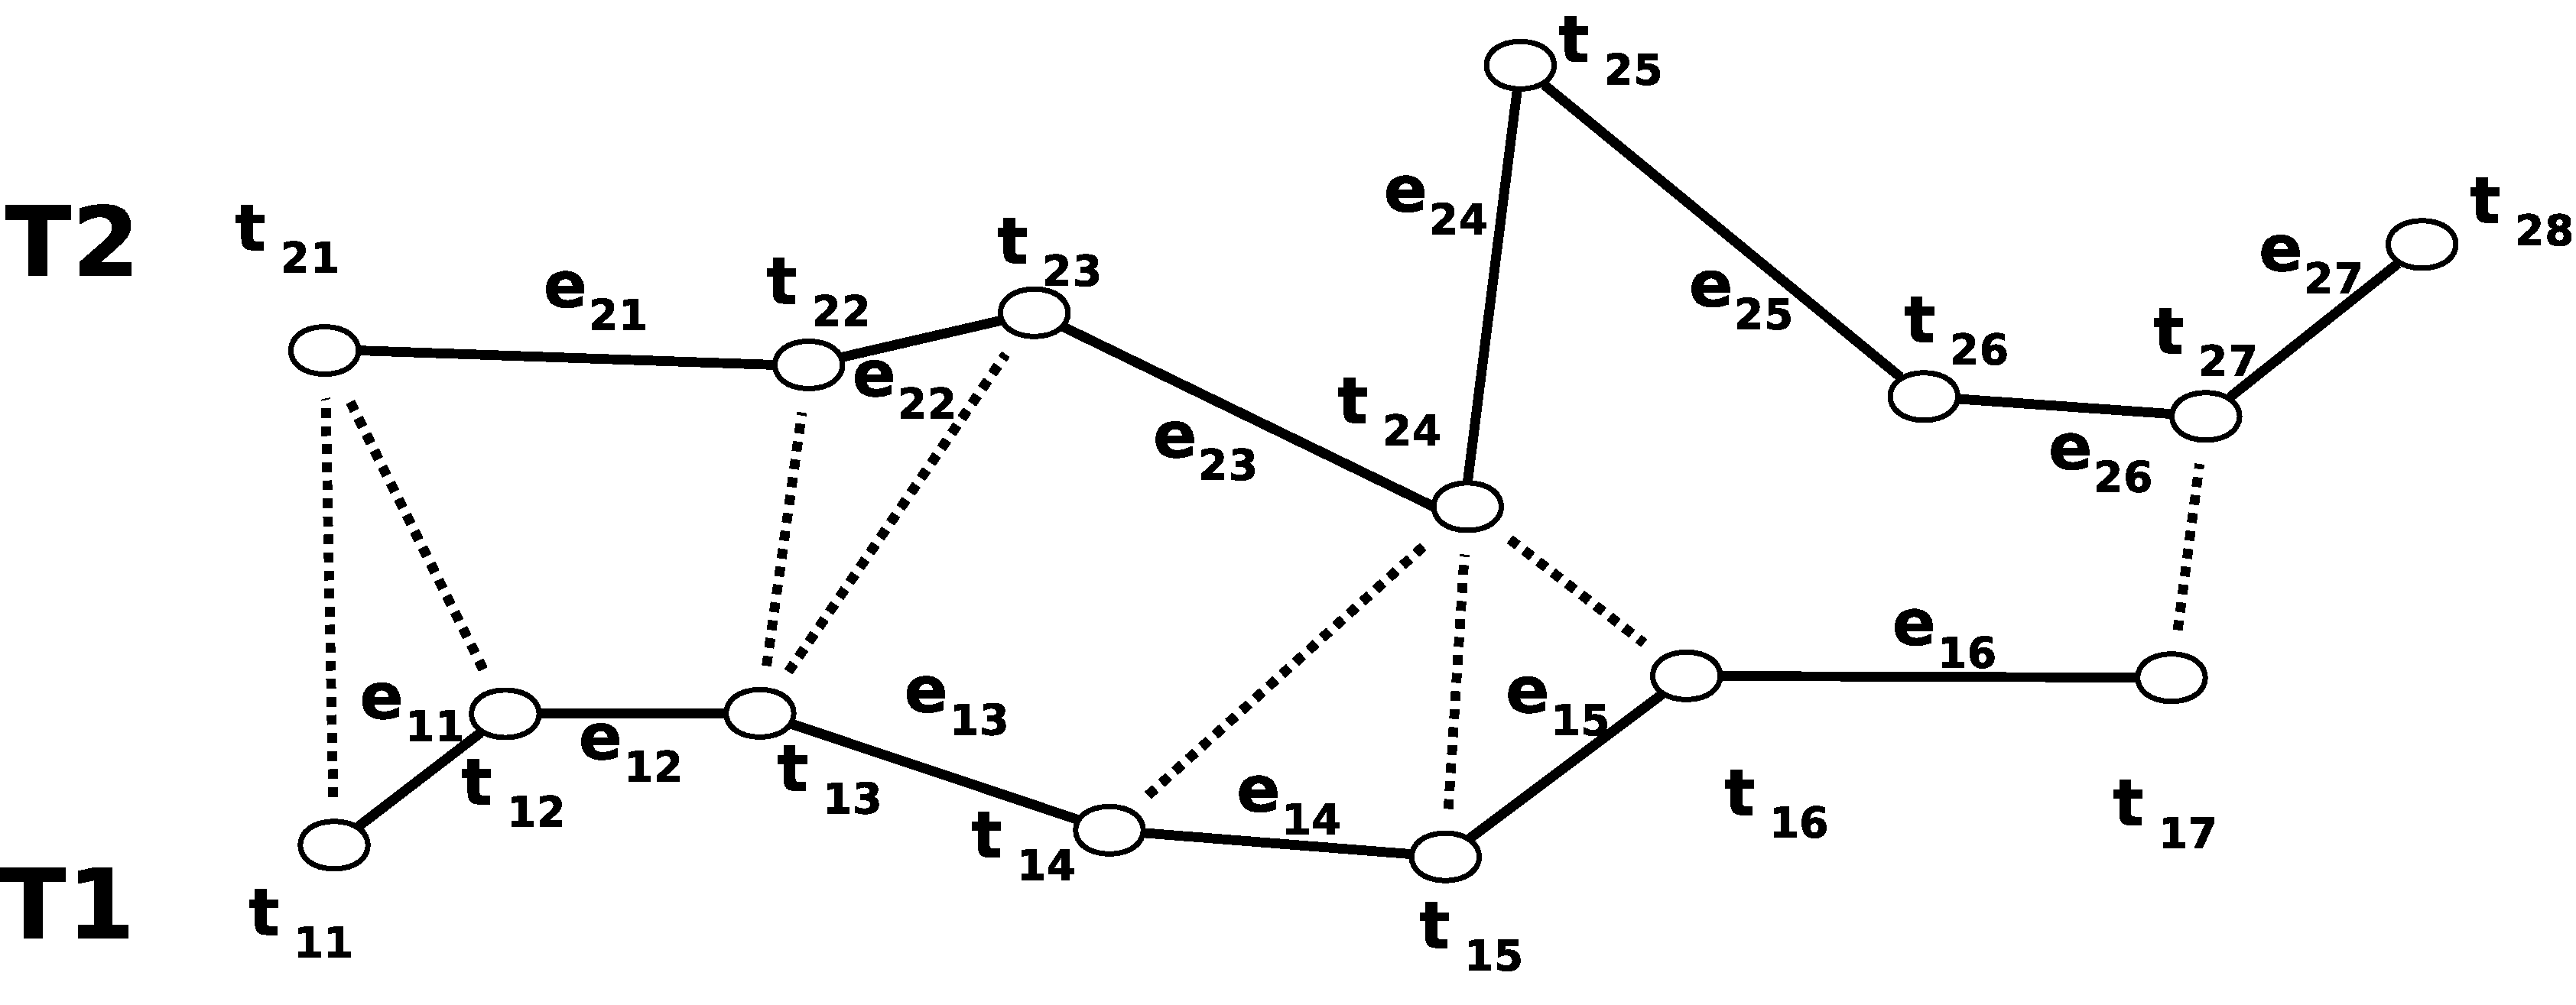
\includegraphics[width=0.5\textwidth]{figures/edgeAlignment2} \\\hline
	{\bf(A)} \\
	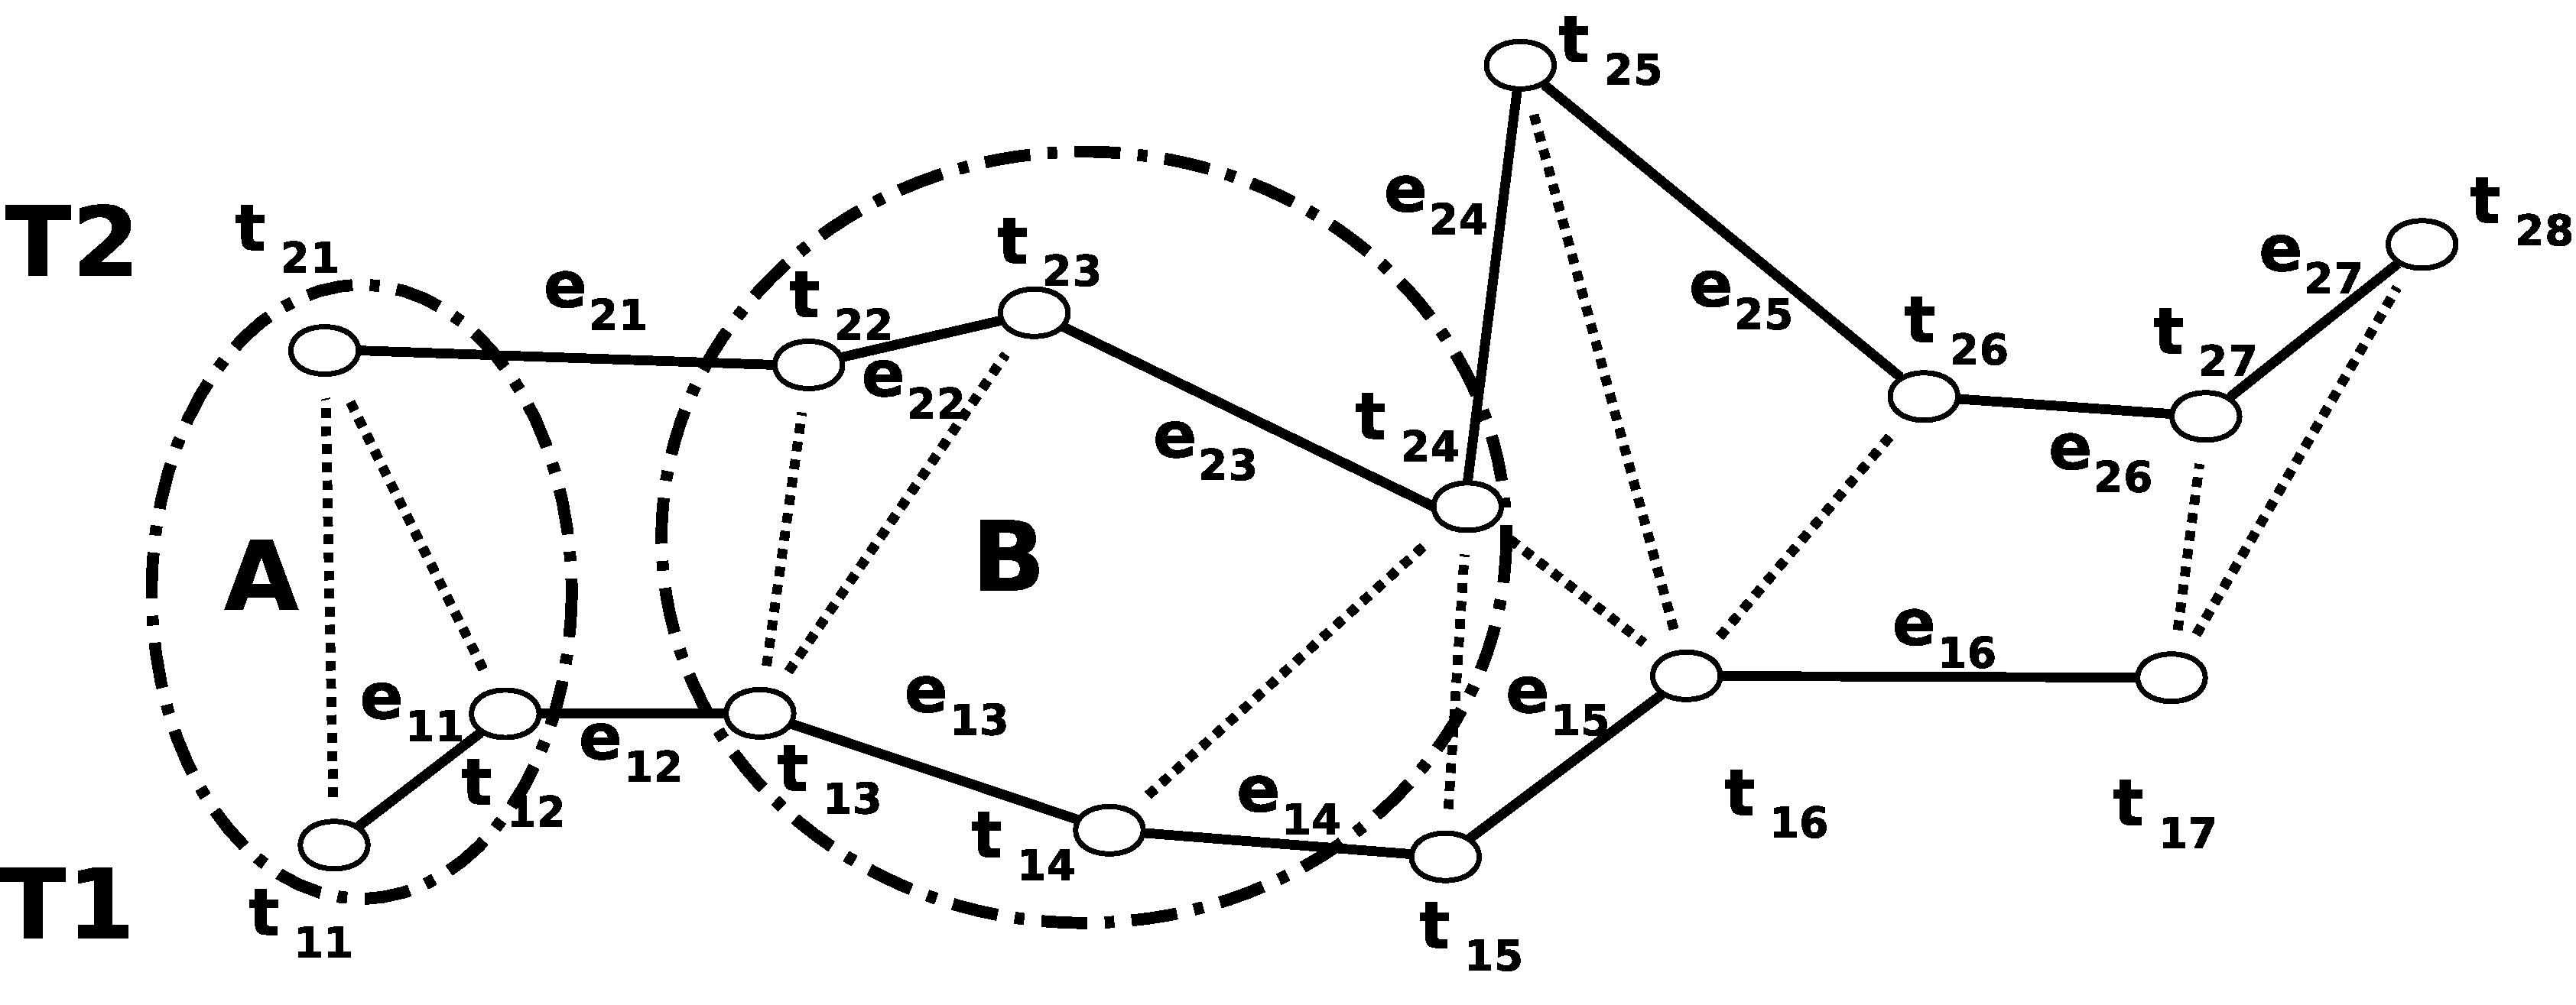
\includegraphics[width=0.5\textwidth]{figures/edgeAlignment3} \\\hline
	{\bf(B)}
  \end{tabular}
  \caption{Edge Alignment when comparing two trajectories}
  \label{fig:edgeAlign}
\end{figure}

\begin{equation}\label{eq:cEdge}
N_{edge}(a,b,c,d) = Min\left(| ac | + | bd |, | ad | +| bc | \right)
\end{equation} 

\begin{equation}\label{eq:dEdge}
d(e_{1}, e_{2}) = | N_{edge}(e_1.v_s, e_1.v_e, e_2.v_s, e_2.v_e) |
\end{equation} 

\begin{equation}\label{eq:ediff}
e_{diff}(e_1,e_2) = \left( \frac{d\left(e_{1}, e_{2}\right)}{2} \right) * (1+|e_{1_{RT}} - e_{2_{RT}}|)
\end{equation}


\begin{equation}\label{eq:tdiff}
\;t_{diff}(t_1,t_2) = \frac{\sum_{\substack{k=1}}^m e_{diff}(t_1.e_k, t_2.e_k)}{m}
\end{equation}



% \begin{equation}\label{eq:rtlimit}
%  \sum_{m=0}^n (|e_{1_m} - e_{2_m}| + (RE_{Before_m} +  RE_{After_m}))
% \end{equation}


\begin{figure}	
\center
	  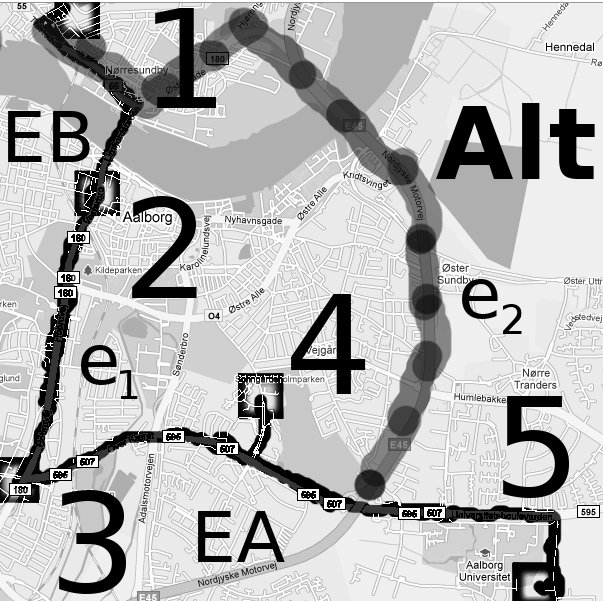
\includegraphics[width=0.2\textwidth]{figures/map2.jpeg}
       \caption{Alternative route}
  \label{fig:altRoute}
\end{figure}


\subsubsection{Timestamp Modification} \label{subsec:timeMod}

% 3 cases:
% 1. connect two trajectories in the \poi, making it seem as one person who never stopped
% 2. redistribute time across edges in the trajectory, making it seem like the user never stopped at the sensitive \poi
% 3. both do detour (in case hospital or other \poi is a small way off a larger road, then just cut away the small detour and patch up the trajectory.

As described in section \ref{subsec:protectiontypes}, when trying to protect a location which is on, or very near, a major road, one possible way of protecting the user is to simply make it look like the user never stopped and just drove right by the location. Figure~\ref{fig:adjustTrajec}A shows on the left side a sample trajectory with start-/end-time for each edge plus time not moving while the user has stopped at the hospital (here assumed to be defined as temporally sensitive). The graph on the right side of figure~\ref{fig:adjustTrajec} shows the distance the user has moved on the vertical axis and the time spent travelling on the horizontal axis. It can clearly be seen on the line for "Not Time adjusted (A)" that the user stops for an hour.

Figure~\ref{fig:adjustTrajec}B shows how the visit to the hospital can be removed simply by redistributing the time spent at the hospital onto the remaining edges on the trajectory, keeping in mind any limitations imposed by traffic or \rt (e.g. speed limits or road conditions). In the graph of figure~\ref{fig:adjustTrajec}, looking at the line for "Time adjusted (B)", it it now looks like the user just drove the entire length of the trajectory without stopping (in this case also at a fairly consistent speed).
The challenge is making sure that the travel times on the individual road-edges is still plausible after modifying the start-/end-times of some or all the road-edges. It can be insured using information about speed limits and average speeds the \rt (Sec.~\ref{subsec:roadtypes}) of the edges in the trajectory. In the example from figure~\ref{fig:adjustTrajec} the start and end times of the trajectory as whole has not been modified, but this is of cause an option but not described further in the algorithm. Adjusting the start and end times of a full trajectory allows for greater flexibility in case it is otherwise impossible to ensure a trajectory is destitute of all information relating to a stop at a sensitive location.


\begin{figure}	
       \center
       \begin{tabular}{cc}
		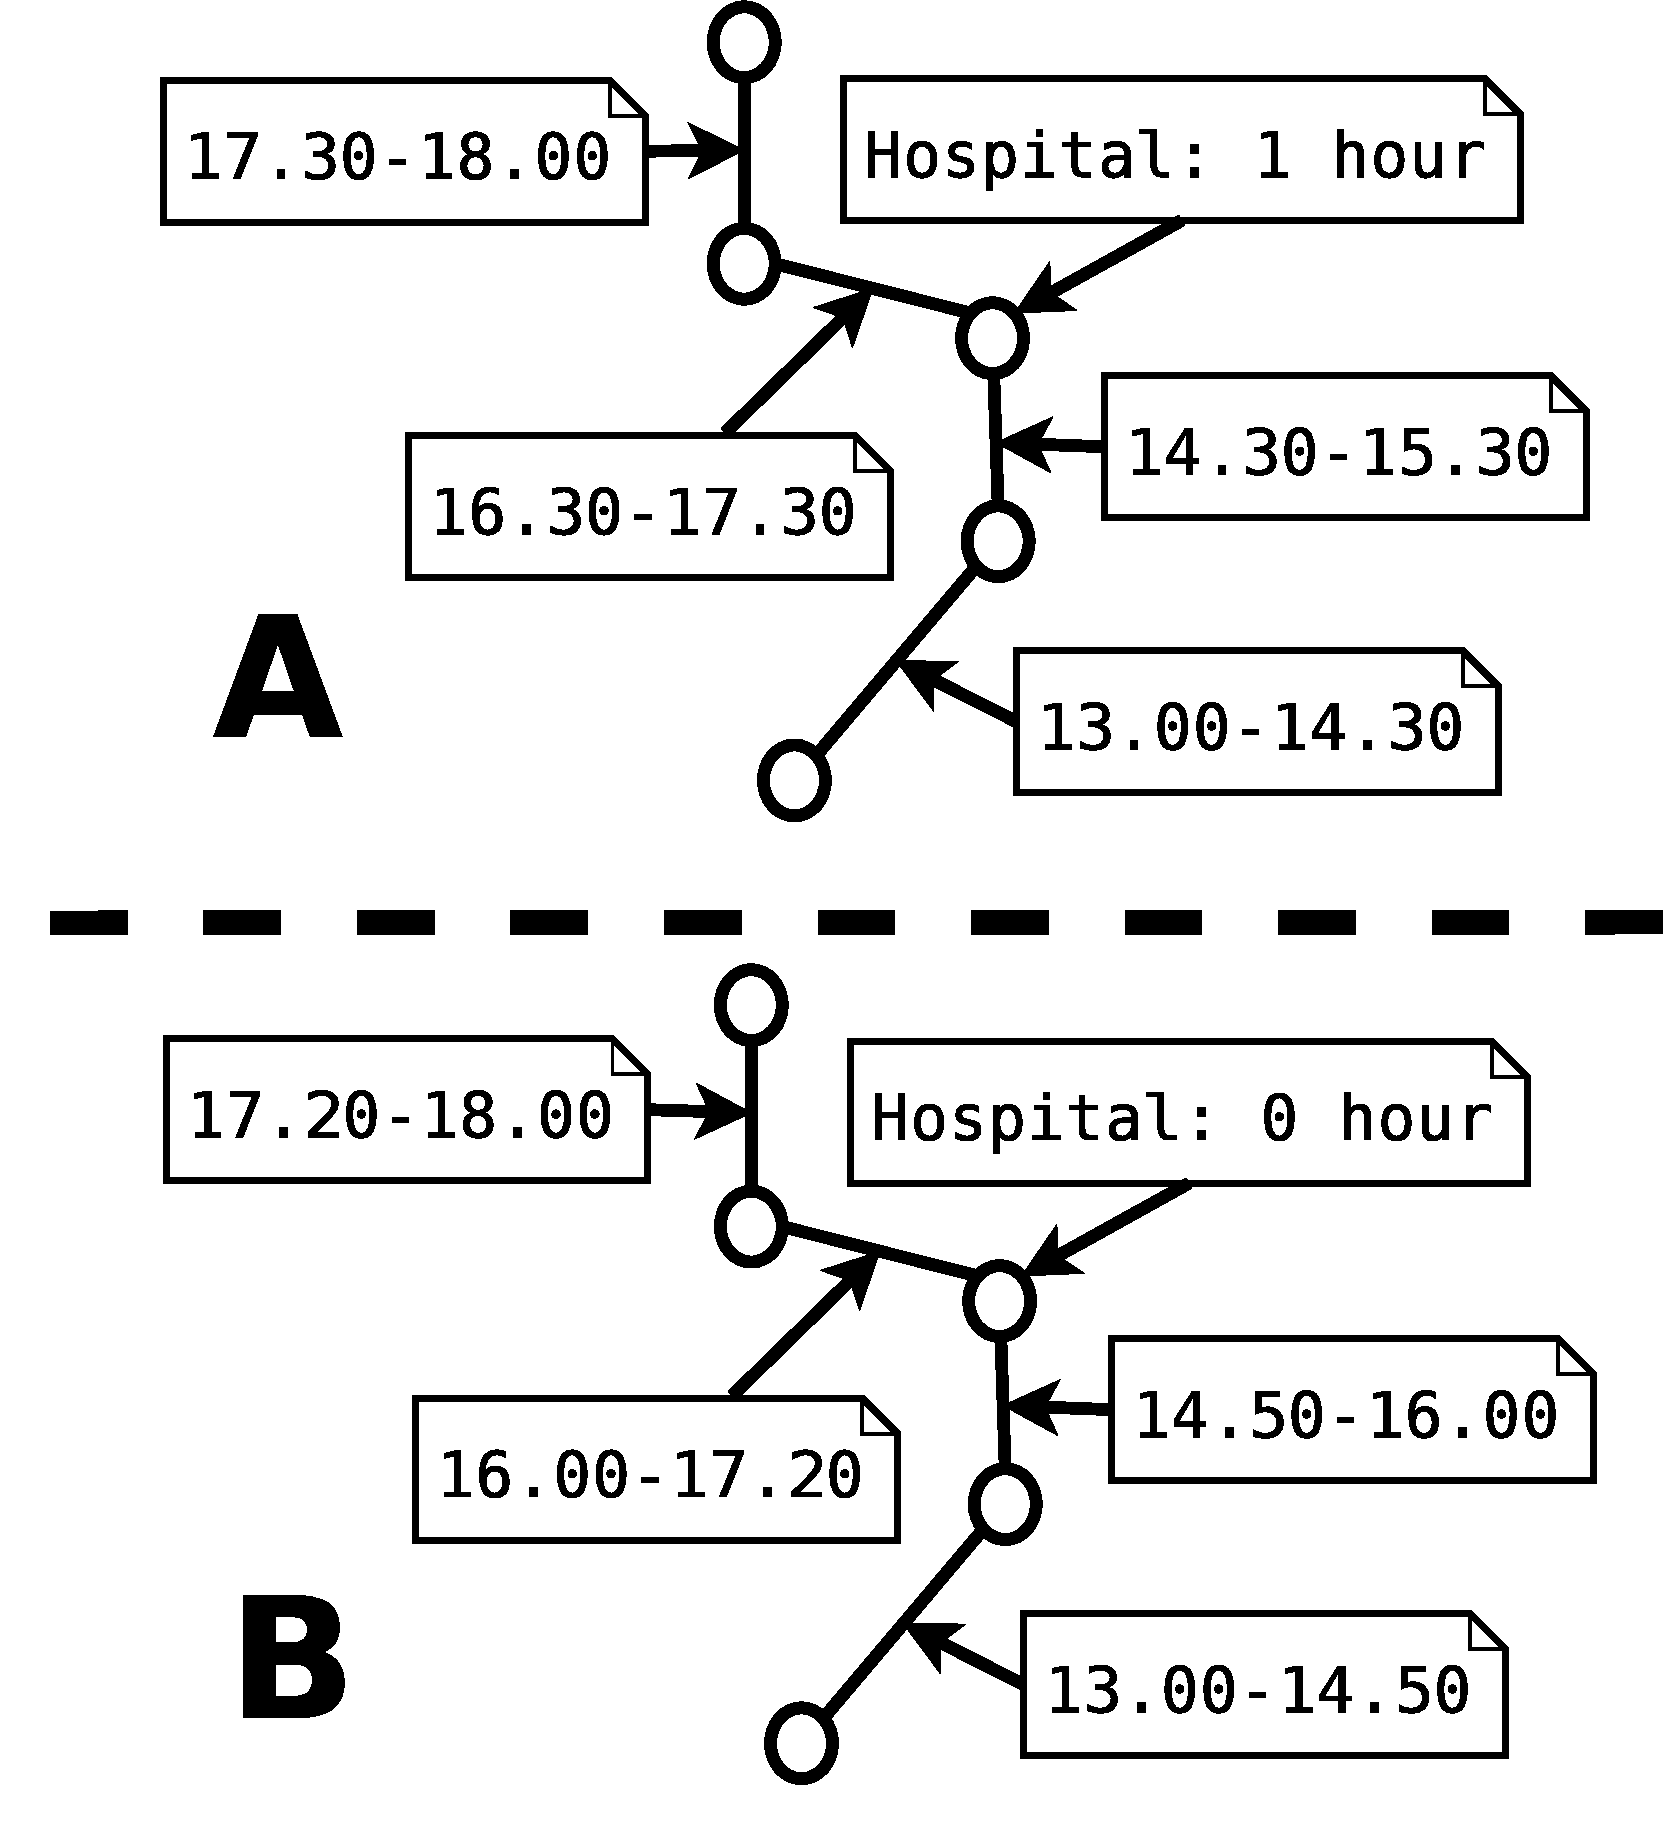
\includegraphics[width=0.20\textwidth]{figures/trajecAdjustTime.pdf} &
		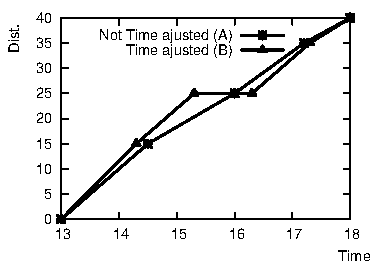
\includegraphics[width=0.25\textwidth]{figures/trajecAdjustTimeGraph.pdf} \\
	\end{tabular}
       \caption{Removal of visit to a hospital by distribution of time onto the road-segments of trajectory.}
  \label{fig:adjustTrajec}
\end{figure}



\subsection{Algorithm}

The algorithm consist of 5 parts, algorithm \ref{alg:overall} is the "master" algorithm which gives a good idea of the control flow in the algorithm, and 4 supporting algorithms, each handling a clearly defined step in algorithm \ref{alg:overall}. In most of the algorithms we work with a 4-tuple: $(t, t_{se}, d_{t}, d_{s})$ consisting of a trajectory, the set of edges in \(t\) defined as sensitive by a \poi and the temporal and spatial sensitivity values from the same \poins. The while loop in algorithm \ref{alg:overall} functions as the main control loop, only ending when there are no more unanonymized sub-trajectories left, i.e. trajectories which have some their edges covered by a \poi and which have not yet been included in $anonData$.
The best understanding of the algorithms will be archived by reading them in the numerical order they are presented, as each algorithm, except 1 \& 5, takes the output of the previous algorithm, modifies the data and returns the modified data.

The algorithms presented has a number of limitations introduced for readability and which should not interfere with the understanding of the how the approach works. First it is assumed that there is only one privacy profile per user, second it is assumed that each trajectory is only covered, or partly covered, by a single \poins. Third it is implicitly assumed that the given set of \pois and the trajectories they cover will "fit" according to their spatial and temporal sensitivities in each 4-tuple, such that after termination of the control loop in algorithm~\ref{alg:overall} no edge of any trajectory has been used twice.


\begin{algorithm}[H!bt]
\dontprintsemicolon
\SetVline

\SetKwInOut{Input}{input}\SetKwInOut{Output}{output}\SetKw{Return}{return}

\Input
{

	$G(V,E)$: Graph representation of Map \;
	$\Psi$: The cache \;
	$\mathcal{B}$: Cache budget \;
	
}
\vspace{0.7em}
\tcp{\emph{H Contains the utility score of all possible \spaths in $\mathbf{G(V,E)}$. The \spath is the value $v$ and the utility is the key $k$, $(k, v)$. The heap is sorted on the key.}}
H Initialize Max-Heap \;

\tcp{\emph{Initialially fill H}}

\ForAll{$\spath_{s,t} | s \in V, t \in V, s \neq t$} 
{
    H.push(S$(\chi, \spath_{s,t}, \Psi), \spath_{s,t}$) \;
}


\tcp{\emph{Fill cache}}
\While{$| \Psi | \leq \mathcal{B}$ AND $\spath_{ms}.k \neq 0$ OR $| H | > 0$}
{
	\tcp{\emph{Assign (utility,\spath) pair with the highest utility to $\spath_{ms}$}}
	$ \langle  key_{max},  SP_{max} \rangle \leftarrow$ H.pop() \; 
	\tcp{\emph{Update utility, as previous \spath insertion has changed it}}
	$key_{max} = S(\chi, \spath_{max}, \Psi)$
	\tcp{\emph{H.TopKey() looks at the top (k,v) pair without removing it from the heap}}
	\If{$key_{max} \geq H.TopKey$} 	
	{
	    \If{$( \mathcal{B} - | \Psi | ) \geq | \spath_{max} |$}
	    {
		$\Psi.insert(\spath_{max})$\;
	    }
	}
	\Else
	{
	    H.push(S$(\chi, \spath_{max}, \Psi), \spath_{max}$) \;
	}
}

\caption{\salgons($G(V,E), \Psi, \mathcal{B}$)}
\label{alg:greedy}
\end{algorithm}

The input to algorithm~\ref{alg:overall} contains all the concepts and parameters introduced in section~\ref{sec:problemdef} and \ref{sec:contribution} and it works as the main control loop, calling subsequent algorithms to anonymize sensitive edges in the set of trajectories \(\mathbf{T}\). The dataflow is such that each call to any of the four other algorithms provide a transformation on the input such that the output is can be used as the input for the next algorithm called.
The main while loop starts by choosing \(\alpha\), a tuple with trajectory containing a number of high sensitivity edges according to a \poi and calls the remaining algorithms on the basis of the chosen \(\alpha\). To choose \(\alpha\) the algorithm will handle the \poi types in the order given by table~\ref{tab:poiclass1} from top to bottom. \pois in each class will also be sorted according to their sensitivity values. The point in doing the \pois in order is that we want to ensure that all \poi are anonymized up to the highest level specified by a user with the least amount of work e.g. given two identical trajectories, one with sensitive endpoints and one without, it is important to choose the one with sensitive endpoints first as it is harder to anonymize and we therefor want to have as many candidates as possible to help anonymize that trajectory first.

The main loop ends when the privacy requirements of all \poi have been covered by some trajectories and ${\bf Choose\_\alpha}$ therefor can no longer find new tuples.
At the end of the main control loop all edges which has not been involved in the anonymization process is added to the anonymized dataset to have a complete dataset after anonymization.



\begin{algorithm}[H!bt]
\dontprintsemicolon
\SetVline

\SetKwInOut{Input}{input}\SetKwInOut{Output}{output}\SetKw{Return}{return}



\Input{
	$\mathbf{\spath_{s,t}}$: A \spath.\;
}

\Output{
	An integer representing the score
}



 \funcc{Score}{\spath_{s,t}}
{
	\textbf{H}.push($S(\chi, SP_{s,t}, \Psi), SP_{s,t}$) \;
% 	\ForEach{edge $e \in \alpha.t$}
% 	{
% 		\ForEach {$psr \in PS$ }
% 		{
% 			\If{$e \in psr.p_{edges}$}
% 			{
% 				${\poins}cand \leftarrow {\poins}cand \cup psr$\;
% 			}
% 		} 
% 	}
}

\caption{Score() function using statistics}
\label{alg:score}
\end{algorithm}

Algorithm~\ref{alg:findCan} finds the set of \poi which cover edges in \(\alpha.t_{se}\). The \poi set is needed to identify the set of trajectories which have edges with sensitivity values similar to \(\alpha\) in algorithm~\ref{alg:calcCan}. 

\begin{figure}	
       \center
	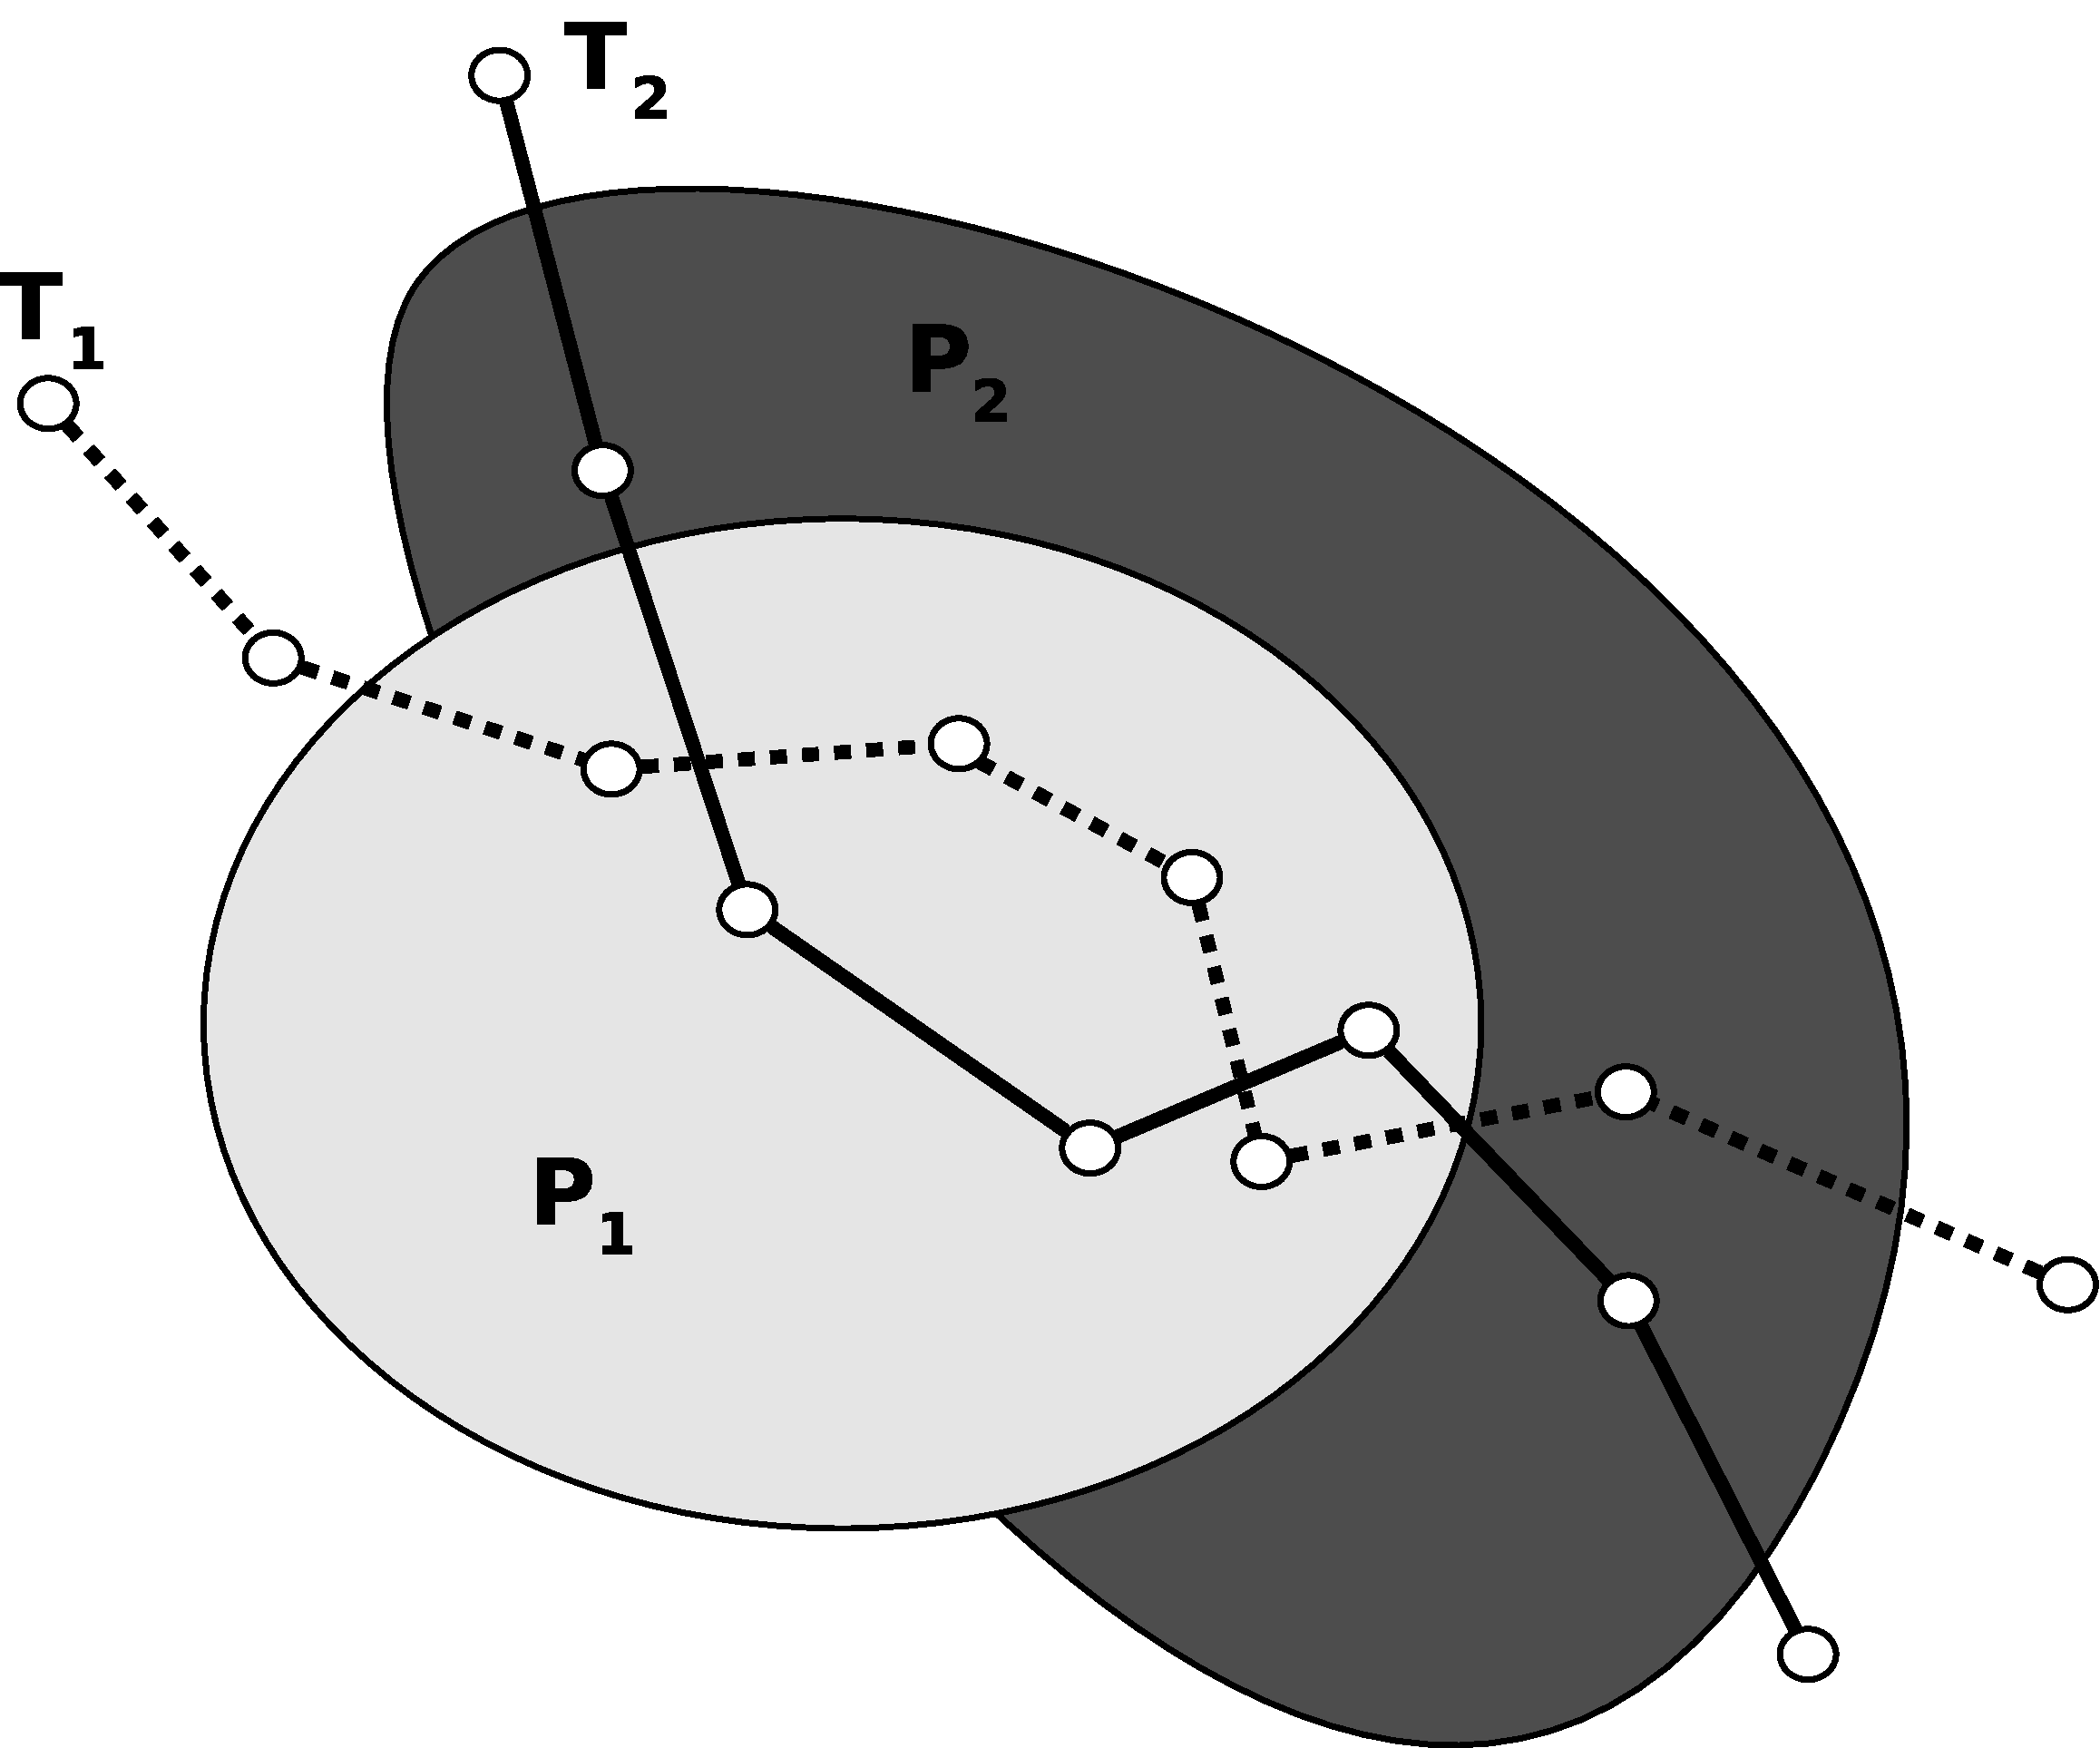
\includegraphics[width=0.40\textwidth]{figures/poiIntersect.pdf} 
       \caption{Two intersecting \poisns. $P_2$ covering all of $T_2$ edges, $P_1$ only covering some of $T_1$ edges. some edges in $T_1$ \& $T_2$ is covered by both \poins.}
  \label{fig:poiOverlap}
\end{figure}



\begin{algorithm}%[H!bt]

\dontprintsemicolon
\SetVline

\SetKwInOut{Input}{input}\SetKwInOut{Output}{output}\SetKw{Return}{return}


\Input{	$\mathbf{T}:$ The set of trajectories. \;

	\(t \in tCand:\) a tuple \((t, t_{se},t.d_t,t.d_s)\)

	$D \in \mathbb{R}$: Tolerance for how much a modified trajectory is allowed to diveate from original trajectory. \;

	$n \in \mathbb{N}$: Granularity of the road difference calculations. \;

	$\alpha$: a tuple $(t, t_{se}, d_{t}, d_{s})$  used as a base for anonymization.\;
}
\Output{

	$calcCand$: set containing calculated alternative trajectories along with their spatial and temporal sensitivity\;
}


\funcc{CalcAlt}{\alpha, t, D, n}
{
	$dLimit \leftarrow 0, diff \leftarrow 0, fail \leftarrow 0$ \;
	$j \leftarrow 1$ \;
	\(calcCand \leftarrow \emptyset\) \;


	$tmpT \leftarrow t.t \setminus \alpha.t$ \tcp{\emph{Ordered set}} \;
	

 	\While{$dLimit \leq D \wedge tmpT \backslash \alpha \neq \emptyset \wedge fail < 2$}
 	{
		%From the shared edges between $\alpha.t$ and $t.t$ choose edges alternating at each end of the shared edges.

		Choose edges alternating at each end of $tmpT$

		edge $e_1 \leftarrow \alpha.t[j]$ \;
		edge $e_2 \leftarrow {\bf closestEdge}(\alpha.t[j], t)$ \;

		\If{$\frac{e_{diff}(e_1,e_2,n) + diff}{j} \leq D$}
		{
			$diff \leftarrow e_{diff}(e_1,e_2,n) + diff$ \;
			$dLimit \leftarrow \frac{diff}{j}$ \;
			$tmpT \leftarrow tmpT \cup \{e_1\}$ \;
			$fail \leftarrow 0$ \;
		} 
		\Else
		{
			$fail \leftarrow fail + 1$ \;
		}

		$j \leftarrow j+1$ \;
	}

	$calcCand \leftarrow calcCand \cup (tmpT, t_{se},t.d_t,t.d_s)$ \;

}

%{\bf TrajectoryFromPSR($P, \mathbf{T}, \alpha$)} - given $\mathbf{T},\alpha$, and a \poi P {\bf TrajectoryFromPSR} returns a set of tubles {(t, $d_t, d_s$)}, where $t \in \mathbf{T}$ belongs to P and has at least one edge in common with $\alpha$ . $d_t, d_s$ is the temporal and spatial sensitivity of $t$.
\funcc{TrajectoriesPSR}{P, \mathbf{T}, \alpha}
{
	$u \leftarrow$ {\bf {\poi}toUser}(P) \tcp{\emph{user $(id,s,\{t\})$ where $P \in s.\{PSR\}$}} \;
 
 	$tSet \leftarrow \{(t, t_{se}, d_t, d_s) | \forall t \in \mathbf{T} \wedge t \cap \alpha.t \neq \emptyset \wedge P.p_{edges} \cup t \neq \emptyset \wedge t_{se} = \alpha.t \cap t \wedge t \in u.t, d_t = P.d_t, d_s = P.d_s \wedge \forall i,j | \alpha.t_{se}[i]_{\tau_{s}}-\frac{\alpha.d_t}{2} \leq t_{se}[j]_{\tau_{s}} \leq \alpha.t_{se}[i]_{\tau_{s}}+\frac{\alpha.d_t}{2} \}$

 	%$t \in \mathbf{T}$. At least one edge in $t$ is covered by P.$p_{edges}$ and $t \bigcap \alpha \neq \emptyset$. The returned tuple include $d_t,d_s,$ and $t_{se} = \alpha \bigcap t$.
 	\Return {$tSet$}
}

\funcc{CalcCand}{{\poins}cand, \alpha, D, n}
{
	\ForEach{\poi P in {\poins}cand}
	{
		tCand $\leftarrow$ {\bf TrajectoriesPSR($P, \mathbf{T}, \alpha$)} \;

 		\ForEach{$t$ in tCand}
 		{
			{\bf CalcAlt}($\alpha, t, D, n$) \;
 		}
	}

	\Return{calcCand} \;
}

\caption{Calculate Candidates}
\label{alg:calcCan}
\end{algorithm}

Algorithm \ref{alg:calcCan} finds the set of tuples containing trajectories which are covered by \poi with sensitivity values equal or close to $\alpha$. Additionally it assured that $t$ share minimum one edge with $\alpha$ ($t.t \cap \alpha.{t} \neq \emptyset$).
The main part of finding this set of similar tuples consist of modifying $t.t$ upto a limit $\mathbf{D}$ of how much it can deviate from the original trajectory, $\mathbf{D}$ being a system parameter which guaranties a minimum level of data integrity after anonymization. These modifications are done by comparing edges of $t.t$ and $\alpha.{t}$ to calculate the {\it road difference} between the original $t.t$ and the alternative routes calculated. The alternative routes are differing from the original up to a factor of $\mathbf{D}$ in {\it road difference} (Equation~\ref{eq:ediff}). This is done as to perform the be best possible anonymization by having the trajectories as similar as possible in the sensitive sections.

The implementation given for {\bf CalcAlt} assumes one edge from an original trajectory will always correspond to one edge in alternative trajectory. This is done purely for readability, as the algorithm of cause will have to handle comparison of two trajectories with different number of edges (e.g the example in figure \ref{fig:edgeAlign}). The requirement that a candidate needs to share share at least one edge with $\alpha.{t}$ to be considered is done to ease readability as it simplifies the algorithm. It is however not necessary for the idea to work, as long as the initial "shared" edge(s) are relatively close. One example of this could be $T_1$ and $T_2$ in figure \ref{fig:poiOverlap}. While they do not share any edges they follow the same direction relatively close to each other part of the way, namely the part in \poi $P_1$ and thus basically any edge in $P_1$ could serve as a starting point and "shared" edge to perform the trajectory transformations in {\bf CalcAlt}.
% 
% \emph{tmpT: edges from $t$ which are candidates to be modified to follow the path of $\alpha$}
% 
% \emph{$\alpha.t_\alpha[j]$ is j'th edge from $\alpha.t$.}
% 
% \emph{${\bf closestEdge}(\alpha.t[j],t)$ finds the edge closest to $\alpha.t[j]$ in trajectory $t$}



\begin{algorithm}%[H!bt]

\dontprintsemicolon
\SetVline

\SetKwInOut{Input}{input}\SetKwInOut{Output}{output}\SetKw{Return}{return}


\Input{
	calcCand \;
}

\Output{
	sortCand \;
}


\tcp{\emph{Specifies ordering to be used by a sorting algorithm}} \;

\funcc{CompareCand}{p1(t,t_{se},d_{t},d_{s}),p2(t,t_{se},d_{t},d_{s}), \alpha}
{
	\If{$p1.d_t > p2.d_t \wedge p1.d_s > p2.d_s$}
	{
		p1 > p2 \;
	}
	\ElseIf{$p1.d_t < p2.d_t \wedge p1.d_s < p2.d_s$}
	{
		p1 < p2 \;
	}
	\If{$p1.d_t > p2.d_t \wedge p1.d_s < p2.d_s \vee p1.d_t < p2.d_t \wedge p1.d_s > p2.d_s$}
	{
		\If{$p1.d_t+p1.d_s > p2.d_t+p2.d_s$}{p1 > p2 \;}
		\ElseIf{$p1.d_t+p1.d_s = p2.d_t+p2.d_s$}
		{
			%\If{$(p1.d_t \vee p1.d_s) > (p2.d_t \wedge p2.d_s)$}
			\If{$((p1.d_t > p2.d_t \wedge p1.d_t > p2.d_s) \vee (p1.d_s > p2.d_t \wedge p1.d_s > p2.d_s)) $}
			{
				p1 > p2 \;
			}
			%\ElseIf{$(p1.d_t \wedge p1.d_s) < (p2.d_t \vee p2.d_s)$}
			\ElseIf{\(((p2.d_t > p1.d_t \wedge p2.d_t > p1.d_s) \vee (p2.d_s > p1.d_t \wedge p2.d_s > p1.d_s)) \)}
			{
				p1 < p2 \;
			}
			\ElseIf{$\mid p1.t \cap \alpha.t | < |\, p2.t \cap \alpha.t\mid$}
			{
				p1 < p2 \;
			}
			\ElseIf{$\mid p1.t \cap \alpha.t | > |\, p2.t \cap \alpha.t \mid $}
			{
				p1 > p2 \;
			}
			\Else
			{
				p1 = p2 \;
			}
		}
	}
}

\caption{Ordering for Sorting algorithm}
\label{alg:sortCan}
\end{algorithm}

Algorithm \ref{alg:sortCan} provides a numerical ordering which is used to sort the candidate set from algorithm \ref{alg:calcCan} before using it as an input to algorithm \ref{alg:AnonymizeCan}. It works on the same 4-tuples used in the other algorithms.

% \emph{Can be any sort algorithm working on a numerical order.\\ the ordering is given below.}


\begin{algorithm}%[H!bt]
\dontprintsemicolon
\SetVline

\SetKwInOut{Input}{input}\SetKwInOut{Output}{output}\SetKw{Return}{return}

\KwData{
tmpAnonData: holds the anonymized data until it fulfills the privacy requirements\;
	
}

\Input{
	$\alpha$ \;
	sortCand \;
}
\Output{
	\(anonData:\) anonymized dataset based on \(\alpha\)\;
}

\funcc{ExpandTime}{tmpAnonData, \alpha}
{
	Find $\alpha$' a trajectory spatially identical to $\alpha.t$ but all timestamps randomly changed to values laying between $\frac{\alpha.d_t}{2}$ below or above the original timestamps $\alpha.t$, while still adhering to the constraints of the road network. It is assumed external information about traffic and speedlimits on the edges are available. \;

	After finding $\alpha$' change all trajectories in tmpAnonData to match the timestamps of $\alpha$' \;

	\Return{$tmpAnonData$}
}

\funcc{AnonCand}{sortCand, \alpha}
{
	\tcp{\emph{Level of temporal/spatial anonymity archived in anonData}}\;
	$dt \leftarrow 0, ds \leftarrow 0$ \;
	$toBeAdded \leftarrow false$ \;
	$tmpAnonData \leftarrow \emptyset$ \;	

	\While{$dt \leq \alpha.d_{t}  \vee ds \leq \alpha.d_{s}$}
	{
		$tmpTuple \leftarrow sortCand.next()$ \;
 		\If{tmpTuple.$d_t \geq \alpha.d_{t}  \wedge dt \leq \alpha.d_t $ }
		{
			$toBeAdded \leftarrow true$ \;
			$dt \leftarrow dt +1$ \;
		}
		\If{tmpTuple.$d_s \geq \alpha.d_{s} \wedge ds \leq \alpha.d_{s}$}
		{
			$toBeAdded \leftarrow true$ \;
			$ds \leftarrow ds +1$ \;
		}
		\If{toBeAdded}
		{
			\tcp{\emph{Spatial anonymity archived}} \;
			$tmpAnonData \leftarrow tmpAnonData \cup \{tmpTuple.t\}$ \;

		}
	}
	\tcp{\emph{Temporal anonymity archived}} \;
	$tmpAnonData \leftarrow {\bf ExpandTime}(tmpAnonData, \alpha)$ \;
		
	\Return{$anonData \cup tmpAnonData$}
}

\caption{Anonymize Candidates}
\label{alg:AnonymizeCan}
\end{algorithm}

Algorithm \ref{alg:AnonymizeCan} provides the final step to complete the anonymization of $\alpha$ together with similar tuples. To achieve the required values for \tanon it is a simple matter of adding the most similar tuples to $\alpha$ from the sorted set of candidates given as input and afterwards do timestamp modification on the set before returning it. 
It should be noted that while this approach will work on an ideal dataset then there are a likely cases it abstracts away to ensure better readability: the sorted set may not even contain suitable candidates, or not enough, to fulfill the privacy requirements of $\alpha$.



